\documentclass[11pt,a4paper]{report}
\usepackage[textwidth=37em,vmargin=30mm]{geometry}
\usepackage{calc,xunicode,amsmath,amssymb,paralist,enumitem,tabu,booktabs,datetime2,xeCJK,xeCJKfntef,listings}
\usepackage{tocloft,fancyhdr,tcolorbox,xcolor,graphicx,eso-pic,xltxtra,xelatexemoji}

\newcommand{\envyear}[0]{2025}
\newcommand{\envdatestr}[0]{2025-07-05}
\newcommand{\envfinaldir}[0]{webdb/2025/20250705/final}

\usepackage[hidelinks]{hyperref}
\hypersetup{
    colorlinks=false,
    pdfpagemode=FullScreen,
    pdftitle={Web Digest - \envdatestr}
}

\setlength{\cftbeforechapskip}{10pt}
\renewcommand{\cftchapfont}{\rmfamily\bfseries\large\raggedright}
\setlength{\cftbeforesecskip}{2pt}
\renewcommand{\cftsecfont}{\sffamily\small\raggedright}

\setdefaultleftmargin{2em}{2em}{1em}{1em}{1em}{1em}

\usepackage{xeCJK,xeCJKfntef}
\xeCJKsetup{PunctStyle=plain,RubberPunctSkip=false,CJKglue=\strut\hskip 0pt plus 0.1em minus 0.05em,CJKecglue=\strut\hskip 0.22em plus 0.2em}
\XeTeXlinebreaklocale "zh"
\XeTeXlinebreakskip = 0pt


\setmainfont{Brygada 1918}
\setromanfont{Brygada 1918}
\setsansfont{IBM Plex Sans}
\setmonofont{JetBrains Mono NL}
\setCJKmainfont{Noto Serif CJK SC}
\setCJKromanfont{Noto Serif CJK SC}
\setCJKsansfont{Noto Sans CJK SC}
\setCJKmonofont{Noto Sans CJK SC}

\setlength{\parindent}{0pt}
\setlength{\parskip}{8pt}
\linespread{1.15}

\lstset{
	basicstyle=\ttfamily\footnotesize,
	numbersep=5pt,
	backgroundcolor=\color{black!5},
	showspaces=false,
	showstringspaces=false,
	showtabs=false,
	tabsize=2,
	captionpos=b,
	breaklines=true,
	breakatwhitespace=true,
	breakautoindent=true,
	linewidth=\textwidth
}






\newcommand{\coverpic}[2]{
    % argv: itemurl, authorname
    Cover photo by #2~~(\href{#1}{#1})
}
\newcommand{\makeheader}[0]{
    \begin{titlepage}
        % \newgeometry{hmargin=15mm,tmargin=21mm,bmargin=12mm}
        \begin{center}
            
            \rmfamily\scshape
            \fontspec{BaskervilleF}
            \fontspec{Old Standard}
            \fontsize{59pt}{70pt}\selectfont
            WEB\hfill DIGEST
            
            \vfill
            % \vskip 30pt
            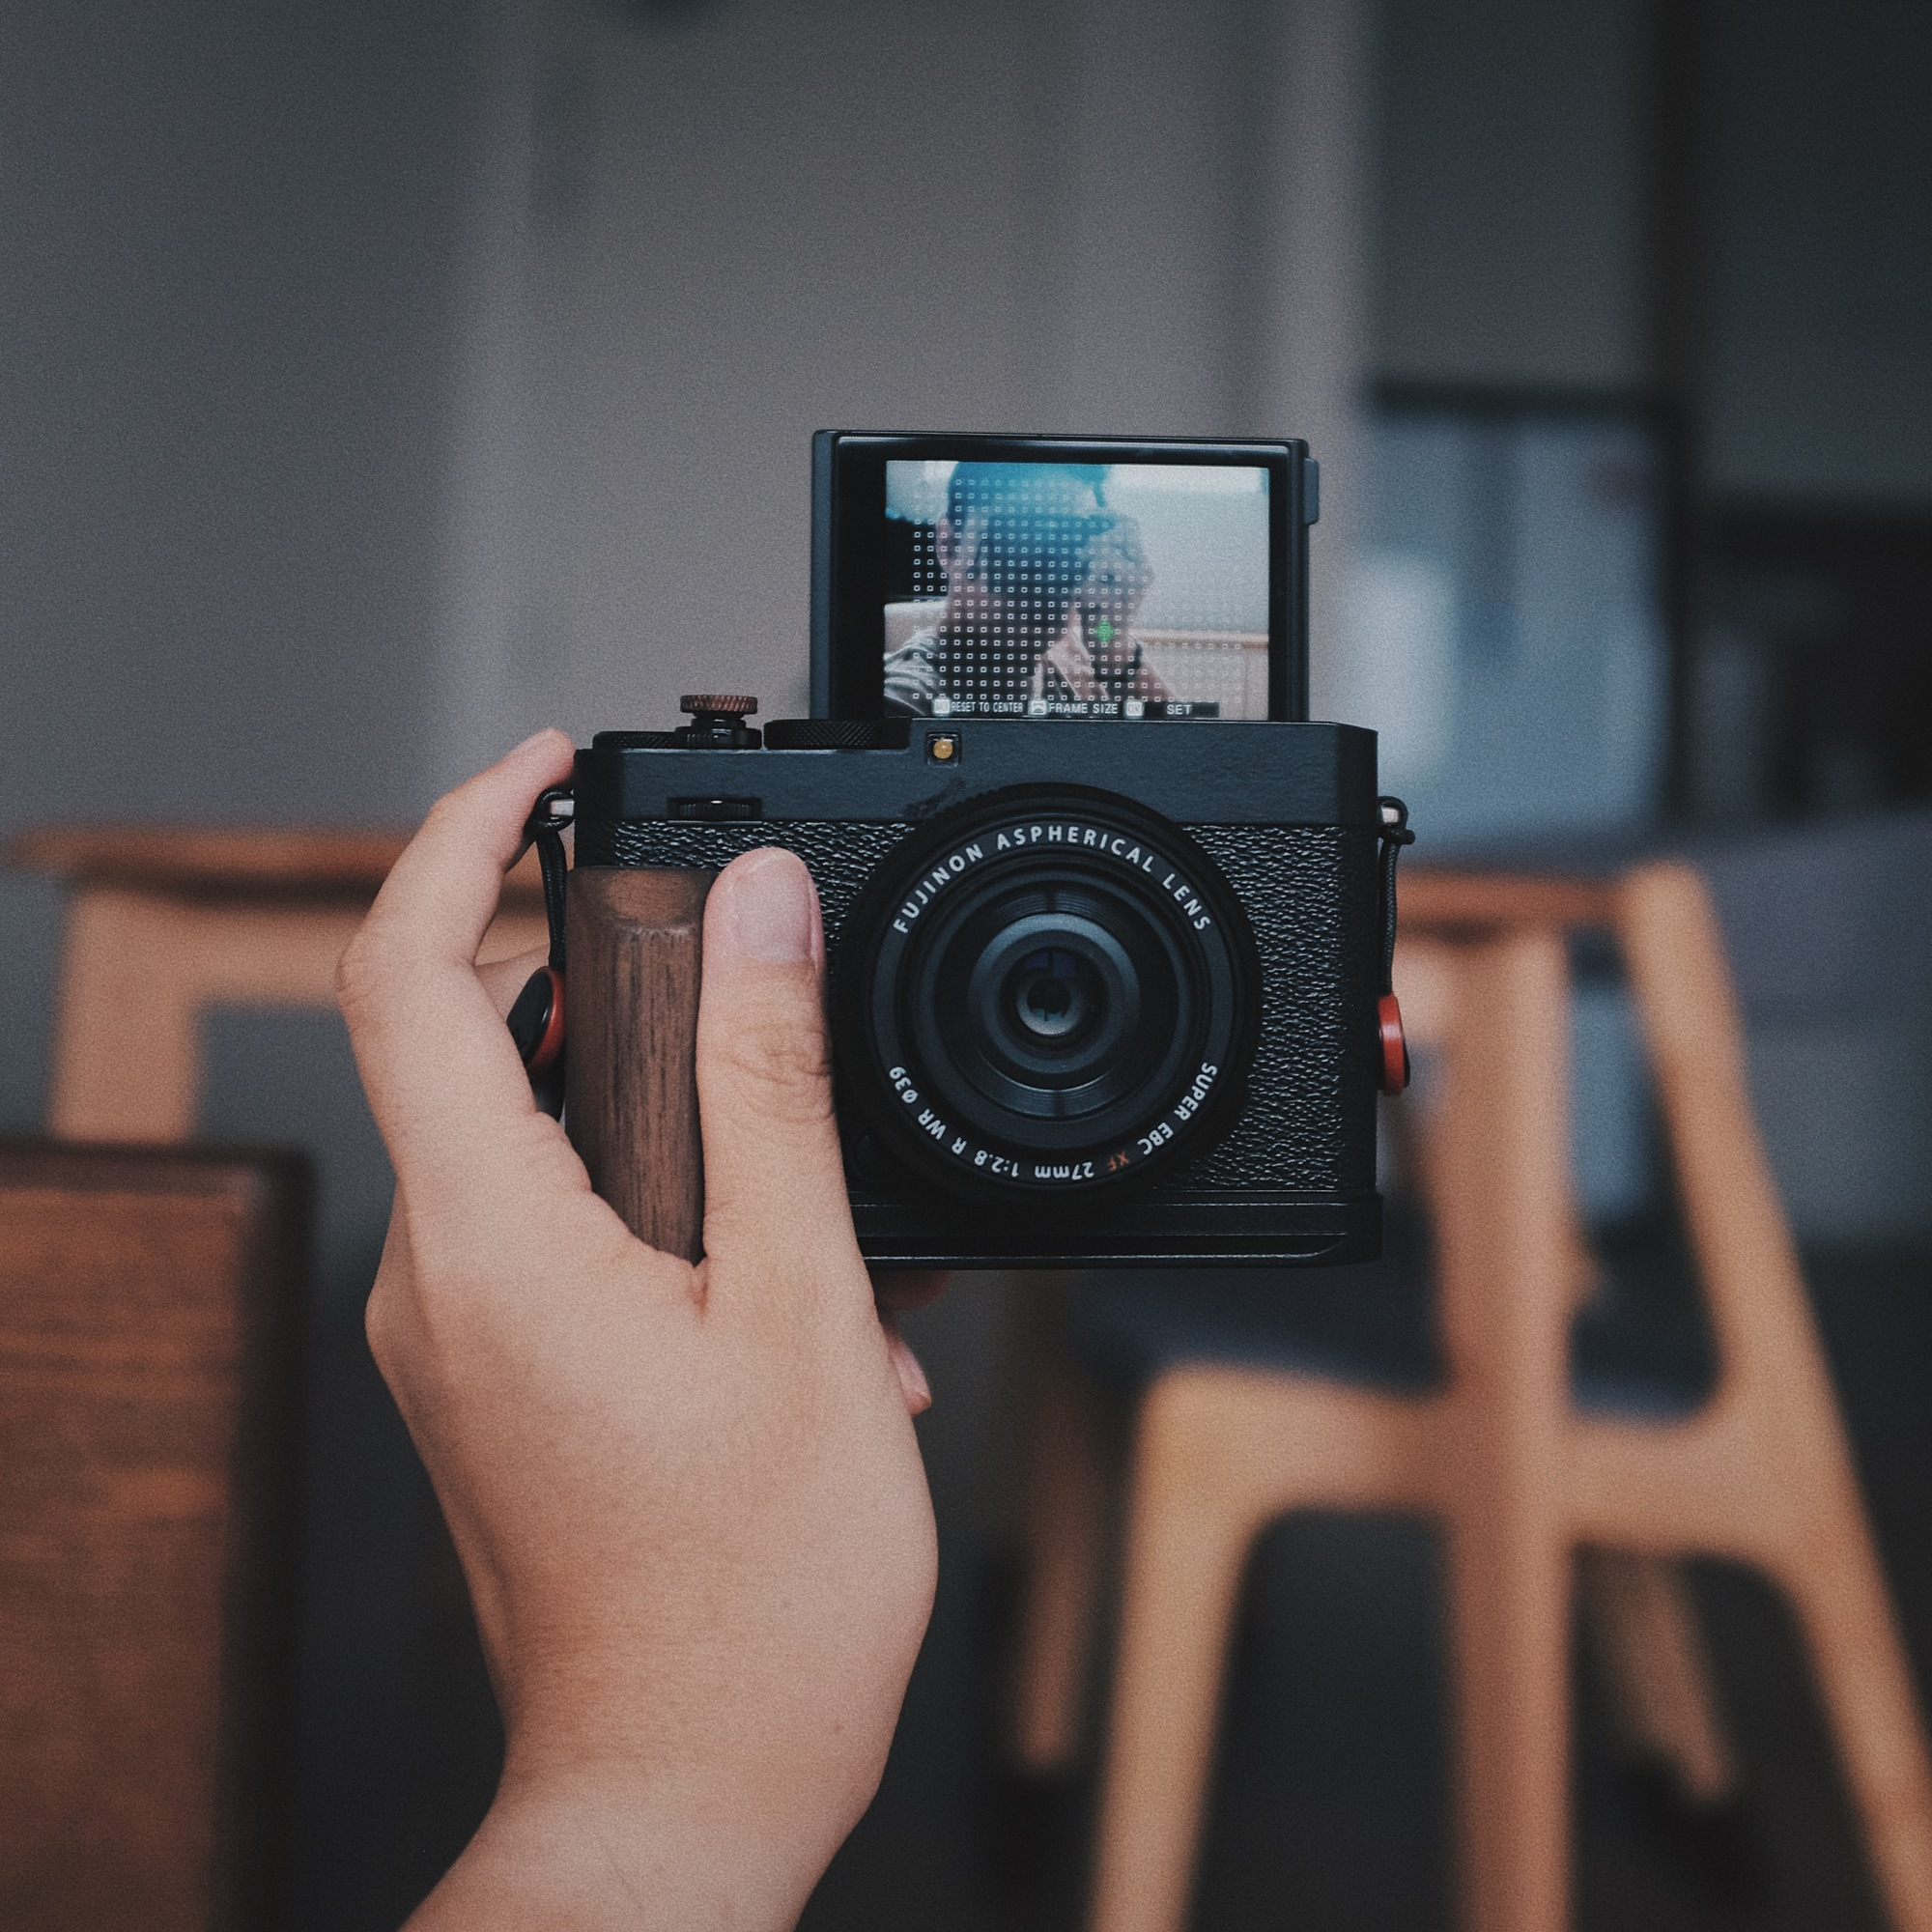
\includegraphics[width=\linewidth]{\envfinaldir/coverpic-prod.jpg}\par
            % \vskip 30pt
            \vfill

            \normalsize\rmfamily\scshape
            \copyright{} The Web Digest Project \hfill\large \envdatestr
        \end{center}
    \end{titlepage}
    % \restoregeometry
}
\newcommand{\simplehref}[1]{%
    \textcolor{blue!80!green}{\href{#1}{#1}}%
}
\renewcommand{\contentsname}{\center\Huge\sffamily\bfseries Contents\par\vskip 20pt}
\newcounter{ipartcounter}
\setcounter{ipartcounter}{0}
\newcommand{\ipart}[1]{
    % \vskip 20pt
    \clearpage
    \stepcounter{ipartcounter}
    \phantomsection
    \addcontentsline{toc}{chapter}{#1}
    % \begin{center}
    %     \Huge
    %     \sffamily\bfseries
    %     #1
    % \end{center}
    % \vskip 20pt plus 7pt
}
\newcounter{ichaptercounter}
\setcounter{ichaptercounter}{0}
\newcommand{\ichapter}[1]{
    % \vskip 20pt
    \clearpage
    \stepcounter{ichaptercounter}
    \phantomsection
    \addcontentsline{toc}{section}{\numberline{\arabic{ichaptercounter}}#1}
    \begin{center}
        \Huge
        \sffamily\bfseries
        #1
    \end{center}
    \vskip 20pt plus 7pt
}
\newcommand{\entrytitlefont}[1]{\subsection*{\raggedright\Large\sffamily\bfseries#1}}
\newcommand{\entryitemGeneric}[2]{
    % argv: title, url
    \parbox{\linewidth}{
        \entrytitlefont{#1}\par\vskip 5pt
        \footnotesize\ttfamily\mdseries
        \simplehref{#2}
    }\vskip 11pt plus 11pt minus 1pt
}
\newcommand{\entryitemGithub}[3]{
    % argv: title, url, desc
    \parbox{\linewidth}{
        \entrytitlefont{#1}\par\vskip 5pt
        \footnotesize\ttfamily\mdseries
        \simplehref{#2}\par\vskip 5pt
        \small\rmfamily\mdseries#3
    }\vskip 11pt plus 11pt minus 1pt
}
\newcommand{\entryitemAp}[3]{
    % argv: title, url, desc
    \parbox{\linewidth}{
        \entrytitlefont{#1}\par\vskip 5pt
        \footnotesize\ttfamily\mdseries
        \simplehref{#2}\par\vskip 5pt
        \small\rmfamily\mdseries#3
    }\vskip 11pt plus 11pt minus 1pt
}
\newcommand{\entryitemHackernews}[3]{
    % argv: title, hnurl, rawurl
    % \parbox{\linewidth}{
    %     \entrytitlefont{#1}\par\vskip 5pt
    %     \footnotesize\ttfamily\mdseries
    %     \simplehref{#3}\par
    %     \textcolor{black!50}{\href{#2}{#2}}
    % }\vskip 11pt plus 11pt minus 1pt
    \begin{minipage}{\linewidth}
            \entrytitlefont{#1}\par\vskip 5pt
            \footnotesize\ttfamily\mdseries
            \simplehref{#3}\par
            \textcolor{black!50}{\href{#2}{#2}}
    \end{minipage}\par\vskip 11pt plus 11pt minus 1pt
}







\begin{document}

\makeheader

\tableofcontents\clearpage




\ipart{Developers}
\ichapter{Hacker News}
\entryitemTwoLinks{Nvidia Is Full of Shit}{https://news.ycombinator.com/item?id=44468175}{https://blog.sebin-nyshkim.net/posts/nvidia-is-full-of-shit/}

\entryitemTwoLinks{Everything around LLMs is still magical and wishful thinking}{https://news.ycombinator.com/item?id=44467949}{https://dmitriid.com/everything-around-llms-is-still-magical-and-wishful-thinking}

\entryitemTwoLinks{Eight dormant Satoshi-era Bitcoin wallets reactivated after 14 yrs}{https://news.ycombinator.com/item?id=44466896}{https://twitter.com/WatcherGuru/status/1941167512491864554}

\entryitemTwoLinks{Air pollution may contribute to development of lung cancer in never-smokers}{https://news.ycombinator.com/item?id=44466838}{https://today.ucsd.edu/story/air-pollution-may-contribute-to-development-of-lung-cancer-in-never-smokers-new-study-finds}

\entryitemTwoLinks{ChatGPT creates phisher's paradise by serving the wrong URLs for major companies}{https://news.ycombinator.com/item?id=44466826}{https://www.theregister.com/2025/07/03/ai\_phishing\_websites/}

\entryitemTwoLinks{How to Incapacitate Google Tag Manager and Why You Should (2022)}{https://news.ycombinator.com/item?id=44466697}{https://backlit.neocities.org/incapacitate-google-tag-manager}

\entryitemTwoLinks{EverQuest}{https://news.ycombinator.com/item?id=44465731}{https://www.filfre.net/2025/07/everquest/}

\entryitemTwoLinks{Mini NASes marry NVMe to Intel's efficient chip}{https://news.ycombinator.com/item?id=44465319}{https://www.jeffgeerling.com/blog/2025/mini-nases-marry-nvme-intels-efficient-chip}

\entryitemTwoLinks{We're not innovating, we're just forgetting slower}{https://news.ycombinator.com/item?id=44464756}{https://www.elektormagazine.com/articles/opinion-no-innovation-forgetting-slower}

\entryitemTwoLinks{I want to leave tech: what do I do?}{https://news.ycombinator.com/item?id=44464647}{https://write.as/conjure-utopia/lets-say-youre-working-in-tech-and-you-have-a-technical-role-youre-a}

\entryitemTwoLinks{Kepler.gl}{https://news.ycombinator.com/item?id=44464641}{https://kepler.gl/}

\entryitemTwoLinks{Serving 200M requests per day with a CGI-bin}{https://news.ycombinator.com/item?id=44464272}{https://jacob.gold/posts/serving-200-million-requests-with-cgi-bin/}

\entryitemTwoLinks{Why I left my tech job to work on chronic pain}{https://news.ycombinator.com/item?id=44464068}{https://sailhealth.substack.com/p/why-i-left-my-tech-job-to-work-on}

\entryitemTwoLinks{Show HN: I AI-coded a tower defense game and documented the whole process}{https://news.ycombinator.com/item?id=44463967}{https://github.com/maciej-trebacz/tower-of-time-game}

\entryitemTwoLinks{Is an Intel N100 or N150 a better value than a Raspberry Pi?}{https://news.ycombinator.com/item?id=44463813}{https://www.jeffgeerling.com/blog/2025/intel-n100-better-value-raspberry-pi}

\entryitemTwoLinks{Larry (cat)}{https://news.ycombinator.com/item?id=44462947}{https://en.wikipedia.org/wiki/Larry\_(cat)}

\entryitemTwoLinks{Writing a Game Boy Emulator in OCaml}{https://news.ycombinator.com/item?id=44462896}{https://linoscope.github.io/writing-a-game-boy-emulator-in-ocaml/}

\entryitemTwoLinks{As a Labrador swam by me out to sea his owner said I hope he doesn't meet a seal}{https://news.ycombinator.com/item?id=44462124}{https://www.irishtimes.com/opinion/an-irish-diary/2025/07/03/all-at-sea-with-a-lockdown-labrador/}

\entryitemTwoLinks{The US dollar is on track for its worst year in modern history}{https://news.ycombinator.com/item?id=44461775}{https://www.semafor.com/article/07/03/2025/the-us-dollar-is-on-track-for-its-worst-year-in-modern-history}

\entryitemTwoLinks{WASM Agents: AI agents running in the browser}{https://news.ycombinator.com/item?id=44461341}{https://blog.mozilla.ai/wasm-agents-ai-agents-running-in-your-browser/}


\ipart{Developers~~~~(zh-Hans)}
\ichapter{Solidot}
\entryitemGeneric{\hskip 0pt{}Stop Killing Games 运动吸引了逾百万人签名}{https://www.solidot.org/story?sid=81721}

\entryitemGeneric{\hskip 0pt{}2024 年发表的医学论文摘要七分之一可能是 AI 完成的}{https://www.solidot.org/story?sid=81720}

\entryitemGeneric{\hskip 0pt{}Clothoff 试图支配深度伪造色情}{https://www.solidot.org/story?sid=81719}

\entryitemGeneric{\hskip 0pt{}基因组测序揭示古埃及人祖先}{https://www.solidot.org/story?sid=81718}

\entryitemGeneric{\hskip 0pt{}海绵结构材料借助太阳热能去除海水中的盐分 }{https://www.solidot.org/story?sid=81717}

\entryitemGeneric{\hskip 0pt{}系外行星引发恒星释放耀斑}{https://www.solidot.org/story?sid=81716}

\entryitemGeneric{\hskip 0pt{}男女对婴儿晚上哭泣声音的反应差别不大}{https://www.solidot.org/story?sid=81715}

\entryitemGeneric{\hskip 0pt{}美国年轻人减少了游戏开支}{https://www.solidot.org/story?sid=81714}

\entryitemGeneric{\hskip 0pt{}TikTok 涌现大量 Google Veo 3 生成的种族主义视频}{https://www.solidot.org/story?sid=81713}

\entryitemGeneric{\hskip 0pt{}微软裁员约九千人,游戏业务深受影响}{https://www.solidot.org/story?sid=81712}

\entryitemGeneric{\hskip 0pt{}天文学家可能发现了已知第三个星际天体}{https://www.solidot.org/story?sid=81711}

\entryitemGeneric{\hskip 0pt{}测试 Firefox 120 到 Firefox 141 在 Linux 下的性能}{https://www.solidot.org/story?sid=81710}

\entryitemGeneric{\hskip 0pt{}任天堂有意锁定 Switch 2 的 USB-C 端口阻止第三方扩展坞}{https://www.solidot.org/story?sid=81709}

\entryitemGeneric{\hskip 0pt{}Copyleft-next 项目重新启动}{https://www.solidot.org/story?sid=81708}

\entryitemGeneric{\hskip 0pt{}西北工业大学成功试飞飞天二号高超音速飞行器}{https://www.solidot.org/story?sid=81707}

\entryitemGeneric{\hskip 0pt{}顶级 AI 工程师的薪水最高超过千万美元}{https://www.solidot.org/story?sid=81706}

\entryitemGeneric{\hskip 0pt{}数据不支持左撇子更具创造力的观点}{https://www.solidot.org/story?sid=81705}

\entryitemGeneric{\hskip 0pt{}OsmAnd 地图应用项目诞生 15 周年}{https://www.solidot.org/story?sid=81704}

\entryitemGeneric{\hskip 0pt{}华为发布了使用昇腾 NPU 训练的开放权重模型}{https://www.solidot.org/story?sid=81703}

\entryitemGeneric{\hskip 0pt{}首批美国科学难民抵达法国}{https://www.solidot.org/story?sid=81702}\ichapter{V2EX}
\entryitemGeneric{\hskip 0pt{}[程序员] 请求大哥们一个抓包问题}{https://www.v2ex.com/t/1143144}

\entryitemGeneric{\hskip 0pt{}[问与答] 不想坐班啊!请大家分享一下不同的工作模式吧!}{https://www.v2ex.com/t/1143143}

\entryitemGeneric{\hskip 0pt{}[酷工作] 远程 flutter 2 名和 vue3 2 名}{https://www.v2ex.com/t/1143142}

\entryitemGeneric{\hskip 0pt{}[程序员] 最佳又迷上了桌搭}{https://www.v2ex.com/t/1143141}

\entryitemGeneric{\hskip 0pt{}[Vercel] 看到 nextjs 的讨论有提到 vercel,想起有个 T-Mobile 的钓鱼站就放在 vercel 上}{https://www.v2ex.com/t/1143139}

\entryitemGeneric{\hskip 0pt{}[问与答] [企业微信] 这个算是企业微信后台的 bug 吗?}{https://www.v2ex.com/t/1143138}

\entryitemGeneric{\hskip 0pt{}[程序员] 分享一个小工具:支持下载 TikTok 视频,无水印 / 高清 / 转音频}{https://www.v2ex.com/t/1143137}

\entryitemGeneric{\hskip 0pt{}[宽带症候群] 听说最近广东和上海的多家中转服务寄了}{https://www.v2ex.com/t/1143136}

\entryitemGeneric{\hskip 0pt{}[酷工作] 招聘远程开发:golang 20k/月起, 有奖金机制,入组配备 ai 工具}{https://www.v2ex.com/t/1143135}

\entryitemGeneric{\hskip 0pt{}[程序员] 记得以前有个项目,在 Docker 创建容器后会得到一个链接,分享给其它人后就可以一起操作运行在 Docker 里面的 Chromium,有没人知道是什么?网页内容都在服务器上渲染}{https://www.v2ex.com/t/1143134}

\entryitemGeneric{\hskip 0pt{}[宽带症候群] 分享一个关于西安电信公网 IP 的事情}{https://www.v2ex.com/t/1143133}

\entryitemGeneric{\hskip 0pt{}[分享发现] 《蓝牙耳机寻回指南》}{https://www.v2ex.com/t/1143132}

\entryitemGeneric{\hskip 0pt{}[汽车] 买车求推荐?}{https://www.v2ex.com/t/1143131}

\entryitemGeneric{\hskip 0pt{}[MacBook Air] Mac Air 有必要上 36G 吗?还是 24G 足够}{https://www.v2ex.com/t/1143130}

\entryitemGeneric{\hskip 0pt{}[问与答] 刚看了冯小刚导演的 1942 电影,河南灾民真惨啊,还有些人是真可恨啊}{https://www.v2ex.com/t/1143129}

\entryitemGeneric{\hskip 0pt{}[分享创造] 用 Cursor 重构了下 bilibili downloader 以及、写小说}{https://www.v2ex.com/t/1143128}

\entryitemGeneric{\hskip 0pt{}[PRO] 优化建议:当只是变化了 active 状态,可以不重新审核}{https://www.v2ex.com/t/1143127}

\entryitemGeneric{\hskip 0pt{}[职场话题] 今天部门开会,我被当众``批评''}{https://www.v2ex.com/t/1143126}

\entryitemGeneric{\hskip 0pt{}[程序员] 大佬们怎么评价盘古与千问的模型纠葛}{https://www.v2ex.com/t/1143122}

\entryitemGeneric{\hskip 0pt{}[站长] 最近入了一个域名,大家参考一下适合做什么站}{https://www.v2ex.com/t/1143120}

\entryitemGeneric{\hskip 0pt{}[分享发现] AI 是牛马的牛马(附庸的附庸不是我的附庸)}{https://www.v2ex.com/t/1143119}

\entryitemGeneric{\hskip 0pt{}[宽带症候群] 江苏、辽宁联通到 Azure 部分 IP 路由不可达}{https://www.v2ex.com/t/1143117}

\entryitemGeneric{\hskip 0pt{}[问与答] 现在这个时间点还建议微信转 wechat 吗}{https://www.v2ex.com/t/1143115}

\entryitemGeneric{\hskip 0pt{}[NAS] 组了台 SAS 硬盘的 NAS}{https://www.v2ex.com/t/1143114}

\entryitemGeneric{\hskip 0pt{}[电动汽车] 小鹏 P7+和 MODEL 3,决赛圈了,懂得车友们说说优缺点吧}{https://www.v2ex.com/t/1143113}

\entryitemGeneric{\hskip 0pt{}[酷工作] 招聘远程全职 IOS,月薪 3500 美金}{https://www.v2ex.com/t/1143112}

\entryitemGeneric{\hskip 0pt{}[酷工作] 招聘远程全职安卓,月薪 3500 美金}{https://www.v2ex.com/t/1143110}

\entryitemGeneric{\hskip 0pt{}[硬件] 想买一款集合 wifi+2.5G 以上的 PCI-E 设备 但似乎没有。}{https://www.v2ex.com/t/1143109}

\entryitemGeneric{\hskip 0pt{}[程序员] 大型多模块 Java 项目你们用什么构建工具}{https://www.v2ex.com/t/1143108}

\entryitemGeneric{\hskip 0pt{}[电动汽车] 避雷小鹏汽车}{https://www.v2ex.com/t/1143107}

\entryitemGeneric{\hskip 0pt{}[奇思妙想] 我会动耳朵,然后我有了一个想法}{https://www.v2ex.com/t/1143103}

\entryitemGeneric{\hskip 0pt{}[问与答] 如何强制关闭网页检测 F12.一打开就自定关闭网页了.}{https://www.v2ex.com/t/1143101}

\entryitemGeneric{\hskip 0pt{}[生活] 网球学习半年花费 1w 了,值吗?}{https://www.v2ex.com/t/1143100}

\entryitemGeneric{\hskip 0pt{}[Python] PythonLink 一个精选优质 Python 资源的导航站}{https://www.v2ex.com/t/1143099}

\entryitemGeneric{\hskip 0pt{}[程序员] 大模型反复犯同一个错误是否和模型精度有关?}{https://www.v2ex.com/t/1143097}

\entryitemGeneric{\hskip 0pt{}[macOS] mac mini 有没有办法自动解锁}{https://www.v2ex.com/t/1143096}

\entryitemGeneric{\hskip 0pt{}[奇思妙想] 如果所有 APP 都能通过截图圈出关键功能来快速定位到相关设置页面就好了。可以快速关闭不需要的功能。}{https://www.v2ex.com/t/1143094}

\entryitemGeneric{\hskip 0pt{}[程序员] 🤪我宣布, 20\$一个月的 vercel 根本就不贵!}{https://www.v2ex.com/t/1143093}

\entryitemGeneric{\hskip 0pt{}[分享创造] 鉴别捞女,拒当龟男,利用 AI 马上搞定}{https://www.v2ex.com/t/1143091}

\entryitemGeneric{\hskip 0pt{}[分享发现] 用文字完整写下自己的想法和困惑,是一件很有帮助的事情}{https://www.v2ex.com/t/1143089}

\entryitemGeneric{\hskip 0pt{}[分享创造] 开源分享:生财有迹(您专属的资产跟踪与分析工具)v3.0 发布}{https://www.v2ex.com/t/1143088}

\entryitemGeneric{\hskip 0pt{}[iPhone] iPhone 16 Pro Max 微信通话,对方听到的声音失真或者听不清}{https://www.v2ex.com/t/1143087}

\entryitemGeneric{\hskip 0pt{}[分享发现] 352 空气净化器联网真是个灾难,不知道有没有 352 内部人员来认领}{https://www.v2ex.com/t/1143086}

\entryitemGeneric{\hskip 0pt{}[问与答] 怎么看待外星系不明物体造访太阳系?}{https://www.v2ex.com/t/1143083}

\entryitemGeneric{\hskip 0pt{}[钓鱼] 竟然有个钓鱼的节点,找杭州的路亚钓友}{https://www.v2ex.com/t/1143082}

\entryitemGeneric{\hskip 0pt{}[Apple] 一个非常好用的快捷指令:快捷进入当前应用的设置界面}{https://www.v2ex.com/t/1143081}

\entryitemGeneric{\hskip 0pt{}[问与答] 有什么办法用上独享 Claude}{https://www.v2ex.com/t/1143080}

\entryitemGeneric{\hskip 0pt{}[深圳] 深圳可以在哪找到育儿嫂?住家阿姨}{https://www.v2ex.com/t/1143078}

\entryitemGeneric{\hskip 0pt{}[问与答] 有用 Ai 辅助玩狼人杀的应用么?}{https://www.v2ex.com/t/1143077}

\entryitemGeneric{\hskip 0pt{}[分享创造] 一键优化生成提示词,我做了个插件来提升写提示词的效率(送会员)}{https://www.v2ex.com/t/1143076}


\ipart{Generic News}







\clearpage
\leavevmode\vfill
\footnotesize

Copyright \copyright{} 2023-2025 Neruthes and other contributors.

This document is published with CC BY-NC-ND 4.0 license.

The entries listed in this newsletter may be copyrighted by their respective creators.

This newsletter is generated by the Web Digest project.

The newsletters are also delivered via Telegram channel \CJKunderline{\href{https://t.me/webdigestchannel}{https://t.me/webdigestchannel}}.\\
RSS feed is available at \CJKunderline{\href{https://webdigest.pages.dev/rss.xml}{https://webdigest.pages.dev/rss.xml}}.

This newsletter is available in PDF at
\CJKunderline{\href{https://webdigest.pages.dev/}{https://webdigest.pages.dev/}}.

The source code being used to generate this newsletter is available at\\
\CJKunderline{\href{https://github.com/neruthes/webdigest}{https://github.com/neruthes/webdigest}}.

This newsletter is also available in
\CJKunderline{\href{http://webdigest.pages.dev/readhtml/\envyear/WebDigest-20250705.html}{HTML}} and
\CJKunderline{\href{https://github.com/neruthes/webdigest/blob/master/markdown/\envyear/WebDigest-20250705.md}{Markdown}}.


\coverpic{https://unsplash.com/photos/a-globular-cluster-shines-brightly-against-the-stars-FsZoT5CQjm0}{Steve Busch}


\end{document}
